

Program analysis and testing go hand in hand to assure the quality of our solutions. For example, running Valgrind becomes more consistent when test code is used. For this reason, we'll configure those two things together. Figure 12.5 illustrates the execution flow and files needed to set them up (a few snippets will be added to the src directory):

\begin{center}
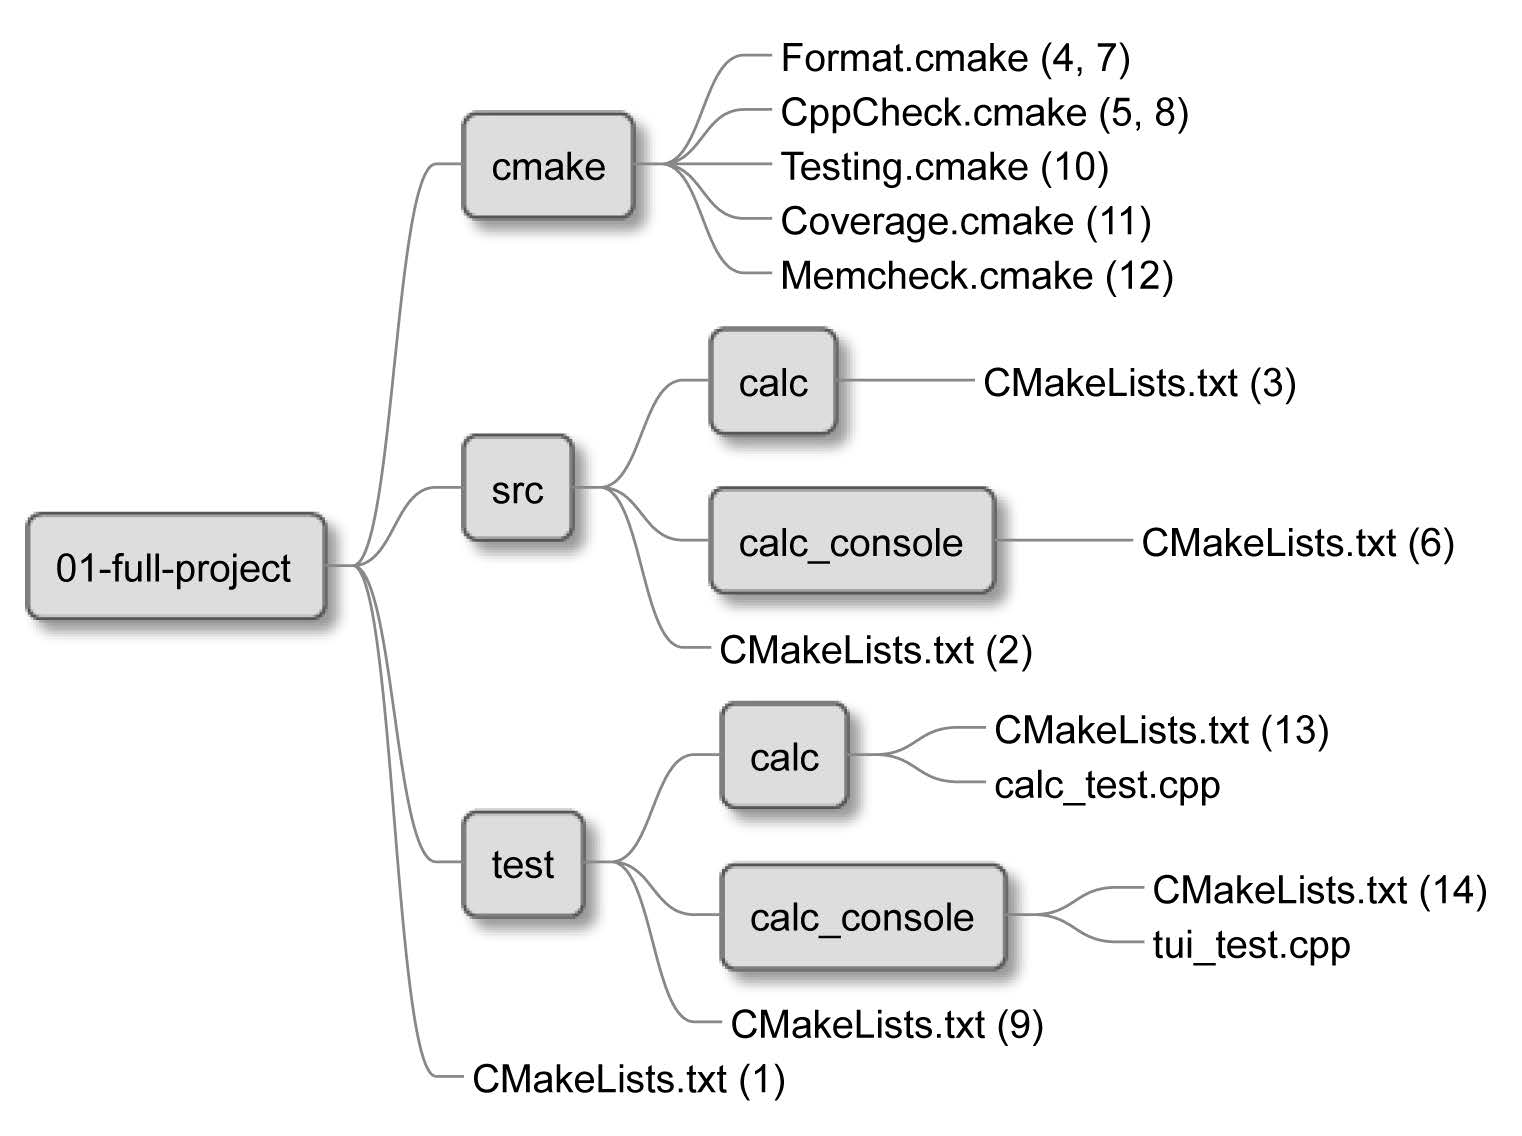
\includegraphics[width=0.8\textwidth]{content/3/chapter12/images/5.jpg}\\
Figure 12.5 – Files used to enable testing and program analysis
\end{center}

As we already know, tests live in the test directory, and their listfile gets executed from the top-level listfile with the add\_subdirectory() command. Let's see what's inside:

\begin{lstlisting}[style=styleCMake]
# chapter-12/01-full-project/test/CMakeLists.txt

include(Testing)
add_subdirectory(calc)
add_subdirectory(calc_console)
\end{lstlisting}

Testing utilities defined in the Testing module are included at this level to allow both target groups (from the calc and the calc\_console directories) to use them:

\begin{lstlisting}[style=styleCMake]
# chapter-12/01-full-project/cmake/Testing.cmake (fragment)

enable_testing()
include(FetchContent)
FetchContent_Declare(
	googletest
	GIT_REPOSITORY https://github.com/google/googletest.git
	GIT_TAG release-1.11.0
)
# For Windows: Prevent overriding the parent project's
# compiler/linker settings
set(gtest_force_shared_crt ON CACHE BOOL "" FORCE)
option(INSTALL_GMOCK "Install GMock" OFF)
option(INSTALL_GTEST "Install GTest" OFF)
FetchContent_MakeAvailable(googletest)
...
\end{lstlisting}

We enabled testing and included the FetchContent module to get GTest and GMock. We're not really using GMock in this project, but these two frameworks are bundled in a single repository, so we need to configure GMock as well. The highlighted part of this configuration disengages the installation of both frameworks from the installation of our project (by setting the appropriate option() to OFF).

Next, we need to create a function that enables the thorough testing of business targets. We'll keep it in the same file:

\begin{lstlisting}[style=styleCMake]
# chapter-12/01-full-project/cmake/Testing.cmake (continued)
...
include(GoogleTest)
include(Coverage)
include(Memcheck)

macro(AddTests target)
	target_link_libraries(${target} PRIVATE gtest_main gmock)
	gtest_discover_tests(${target})
	AddCoverage(${target})
	AddMemcheck(${target})
endmacro()
\end{lstlisting}

Here, we first include the necessary modules: GoogleTest is bundled with CMake, but Coverage and Memcheck will be written by us. We then provide an AddTests macro, which will prepare a target for testing, instrument coverage, and memory checking. Let's see how it works in detail.

\subsubsubsection{12.5.1\hspace{0.2cm}Preparing the coverage module}

Adding coverage to multiple targets is a little bit tricky, as it consists of a few steps. We start by introducing two functions that enable coverage tracking and clean stale tracking files between builds:

\begin{lstlisting}[style=styleCMake]
# chapter-12/01-full-project/cmake/Coverage.cmake (fragment)

function(EnableCoverage target)
	if (CMAKE_BUILD_TYPE STREQUAL Debug)
		target_compile_options(${target} PRIVATE --coverage
			-fno-inline)
		target_link_options(${target} PUBLIC --coverage)
	endif()
endfunction()

function(CleanCoverage target)
	add_custom_command(TARGET ${target} PRE_BUILD COMMAND
		find ${CMAKE_BINARY_DIR} -type f
		-name '*.gcda' -exec rm {} +)
endfunction()
\end{lstlisting}

The preceding functions will be used later, when we get to individual target configurations (calc\_... and calc\_console\_...). The Coverage module will also provide a function that generates the custom coverage target:

\begin{lstlisting}[style=styleCMake]
# chapter-12/01-full-project/cmake/Coverage.cmake (continued)

function(AddCoverage target)
	find_program(LCOV_PATH lcov REQUIRED)
	find_program(GENHTML_PATH genhtml REQUIRED)
	add_custom_target(coverage-${target}
		COMMAND ${LCOV_PATH} -d . --zerocounters
		COMMAND $<TARGET_FILE:${target}>
		COMMAND ${LCOV_PATH} -d . --capture -o coverage.info
		COMMAND ${LCOV_PATH} -r coverage.info '/usr/include/*'
			-o filtered.info
		COMMAND ${GENHTML_PATH} -o coverage-${target}
			filtered.info --legend
		COMMAND rm -rf coverage.info filtered.info
		WORKING_DIRECTORY ${CMAKE_BINARY_DIR}
	)
endfunction()
\end{lstlisting}

AddCoverage() is called in the AddTests() function in the Testing module. It differs slightly from the one introduced in Chapter 8, Testing Frameworks, as it takes the name of the target into account and adds it to the output path to avoid any collisions.

To generate reports for both test targets, we simply need to run two cmake commands (after configuring the project with the Debug build type):

\begin{tcblisting}{commandshell={}}
cmake --build <build-tree> -t coverage-calc_test
cmake --build <build-tree> -t coverage-calc_console_test
\end{tcblisting}

It's now time to modify the Memcheck module that we created earlier (in Chapter 9, Program Analysis Tools) to handle multiple targets.

\subsubsubsection{12.5.2\hspace{0.2cm}Preparing the Memcheck module}

Generation of the Valgrind memory management report is called by AddTests(). We'll start this module with the general setup:

\begin{lstlisting}[style=styleCMake]
# chapter-12/01-full-project/cmake/Memcheck.cmake (fragment)

include(FetchContent)
FetchContent_Declare(
	memcheck-cover
	GIT_REPOSITORY https://github.com/Farigh/memcheckcover.git
	GIT_TAG release-1.2
)
FetchContent_MakeAvailable(memcheck-cover)
\end{lstlisting}

We're familiar with this code already; let's look at the function that'll create appropriate targets for report generation:

\begin{lstlisting}[style=styleCMake]
# chapter-12/01-full-project/cmake/Memcheck.cmake (continued)

function(AddMemcheck target)
	set(MEMCHECK_PATH ${memcheck-cover_SOURCE_DIR}/bin)
	set(REPORT_PATH "${CMAKE_BINARY_DIR}/valgrind-${target}")
	
	add_custom_target(memcheck-${target}
		COMMAND ${MEMCHECK_PATH}/memcheck_runner.sh -o
			"${REPORT_PATH}/report"
			-- $<TARGET_FILE:${target}>
		COMMAND ${MEMCHECK_PATH}/generate_html_report.sh
			-i ${REPORT_PATH}
			-o ${REPORT_PATH}
		WORKING_DIRECTORY ${CMAKE_BINARY_DIR}
	)
endfunction()
\end{lstlisting}

To handle multiple targets, the REPORT\_PATH variable is set to store the path to a targetspecific report. This variable is then used in subsequent commands.

Generation of Memcheck reports can be achieved with following commands (this works better in the Debug build type):

\begin{tcblisting}{commandshell={}}
cmake --build <build-tree> -t memcheck-calc_test
cmake --build <build-tree> -t memcheck-calc_console_test
\end{tcblisting}

These are all modules used by the Testing module. Let's see how it is used.

\subsubsubsection{12.5.3\hspace{0.2cm}Applying testing scenarios}

A few things have to happen for the testing to work:

\begin{enumerate}
\item 
We need to create nested listfiles and define test targets for both directories.

\item 
Unit tests need to be written and prepared as executable targets.

\item 
These targets need to have AddTests() called on them.

\item 
Software Under Test (SUT) needs to be instrumented to enable coverage collection.

\item 
Collected coverage should be cleaned between the builds to avoid segmentation faults.
\end{enumerate}

As implied in test/CMakeLists.txt, we'll create two nested listfiles that configure our tests. Once more, we'll provide one for the library:

\begin{lstlisting}[style=styleCMake]
# chapter-12/01-full-project/test/calc/CMakeLists.txt (fragment)

add_executable(calc_test calc_test.cpp)
target_link_libraries(calc_test PRIVATE calc_static)
AddTests(calc_test)
EnableCoverage(calc_obj)
\end{lstlisting}

We'll also provide one for the executable:

\begin{lstlisting}[style=styleCMake]
# chapter-12/01-full-project/test/calc_console/CMakeLists.txt (fragment)
add_executable(calc_console_test tui_test.cpp)
target_link_libraries(calc_console_test
	PRIVATE calc_console_static)
AddTests(calc_console_test)
EnableCoverage(calc_console_static)
\end{lstlisting}

To keep things brief, we'll provide as simple unit tests as possible. One file will cover the library:

\begin{lstlisting}[style=styleCXX]
// chapter-12/01-full-project/test/calc/calc_test.cpp

#include "calc/calc.h"
#include <gtest/gtest.h>

TEST(CalcTest, SumAddsTwoInts) {
	EXPECT_EQ(4, Calc::Sum(2, 2));
}
TEST(CalcTest, MultiplyMultipliesTwoInts) {
	EXPECT_EQ(12, Calc::Multiply(3, 4));
}
\end{lstlisting}

And we'll have a second file to test the business code. For this purpose, we'll use the FXTUI library. Again, there's no expectation that you will understand this source code in every detail. Test listings are provided in this chapter merely for completeness:

\begin{lstlisting}[style=styleCXX]
// chapter-12/01-full-project/test/calc_console/tui_test.cpp

#include "tui.h"
#include <gmock/gmock.h>
#include <gtest/gtest.h>
#include <ftxui/screen/screen.hpp>
using namespace ::ftxui;

TEST(ConsoleCalcTest, RunWorksWithDefaultValues) {
	auto component = getTui();
	auto document = component->Render();
	auto screen = Screen::Create(Dimension::Fit(document));
	Render(screen, document);
	auto output = screen.ToString();
	ASSERT_THAT(output, testing::HasSubstr("Sum: 102"));
}
\end{lstlisting}

This test code simply renders the textual UI in a default state to a static screen object, which then gets stored in a string. In order for the test to pass, the output needs to contain a substring with the default sum.

Now, we'll need to complete the remaining steps: after we have created test targets and prepared their source code, it's time to register them in CPack with the AddTests() function from the Testing module.

We do this for the library:

\begin{lstlisting}[style=styleCMake]
# chapter-12/01-full-project/test/calc/CMakeLists.txt (continued)

# ... calc_test target definition
AddTests(calc_test)
EnableCoverage(calc_obj)
\end{lstlisting}

We then do it for the executable:

\begin{lstlisting}[style=styleCMake]
# chapter-12/01-full-project/test/calc_console/CMakeLists.txt (continued)

# ... calc_console_test target definition
AddTests(calc_console_test)
EnableCoverage(calc_console_static)
\end{lstlisting}

Subsequently, we instruct the SUT to enable coverage instrumentation with EnableCoverage(). Note that in the case of the library, we had to add instrumentation to the object library rather than the static one. This is because the -{}-coverage flag has to be added to the compilation step, which happens when calc\_obj is being built. Unfortunately, we can't add cleaning of the coverage files here, as CMake requires add\_custom\_command hooks to be called in the same directory as the target definition.

This brings us back to the src/calc and src/calc\_console listfiles that we didn't complete previously. We'll need to add CleanCoverage(calc\_static) and CleanCoverage(calc\_console\_static) respectively (we have to include the Coverage module first). What else needs to be added to these files? Instructions to enable static analysis!

\subsubsubsection{12.5.4\hspace{0.2cm}Adding static analysis tools}

We postponed the continuation of business code listfiles until now so that we can discuss added modules in the appropriate context. We can add a CleanCoverage function call and a few other things to the library listfile:

\begin{lstlisting}[style=styleCMake]
# chapter-12/01-full-project/src/calc/CMakeLists.txt (continued)

# ... calc_static target definition
include(Coverage)
CleanCoverage(calc_static)
include(Format)
Format(calc_static .)
include(CppCheck)
AddCppCheck(calc_obj)
# ... documentation generation
\end{lstlisting}

We can also add them to the executable:

\begin{lstlisting}[style=styleCMake]
# chapter-12/01-full-project/src/calc_console/CMakeLists.cmake (continued)

# ... calc_console_static target definition
include(BuildInfo)
BuildInfo(calc_console_static)
include(Coverage)
CleanCoverage(calc_console_static)
include(Format)
Format(calc_console_static .)
include(CppCheck)
AddCppCheck(calc_console_static)
# ... documentation generation
# ... calc_console bootstrap target definition
\end{lstlisting}

These files are almost complete now (as the second comment suggests, we still need to add the documentation code, which will happen in the Automatic documentation generation section).

Two new modules appear in the listings: Format and CppCheck. Let's dive into the first one:

\begin{lstlisting}[style=styleCMake]
# chapter-12/01-full-project/cmake/Format.cmake

function(Format target directory)
	find_program(CLANG-FORMAT_PATH clang-format REQUIRED)
	set(EXPRESSION h hpp hh c cc cxx cpp)
	list(TRANSFORM EXPRESSION PREPEND "${directory}/*.")
	file(GLOB_RECURSE SOURCE_FILES FOLLOW_SYMLINKS
		LIST_DIRECTORIES false ${EXPRESSION}
	)
	add_custom_command(TARGET ${target} PRE_BUILD COMMAND
		${CLANG-FORMAT_PATH} -i --style=file ${SOURCE_FILES}
	)
endfunction()
\end{lstlisting}

The Format() function is an exact copy of the formatting function described in Chapter 9, Program Analysis Tools; we're simply reusing it here.

Next up is a completely new CppCheck module:

\begin{lstlisting}[style=styleCMake]
# chapter-12/01-full-project/cmake/CppCheck.cmake

function(AddCppCheck target)
	find_program(CPPCHECK_PATH cppcheck REQUIRED)
	set_target_properties(${target}
		PROPERTIES CXX_CPPCHECK
		"${CPPCHECK_PATH};--enable=warning;--error-exitcode=10"
	)
endfunction()
\end{lstlisting}

This is simple and convenient. You may see some resemblance to the Clang-Tidy module (from Chapter 9, Program Analysis Tools); this is CMake's strength – many concepts working the same way. Note the arguments passed to cppcheck:

\begin{itemize}
\item 
-{}-enable=warning – This specifies that we'd like to get warning messages. You can enable additional checks – refer to the Cppcheck manual for more details (the link can be found in the Further reading section).

\item 
-{}-error-exitcode=10 – This specifies that we'd like to get an error code when cppcheck detects an issue. This can be any number from 1 to 255 (as 0 indicates success), although some numbers can be reserved by the system.
\end{itemize}

Usage is very convenient – calling AddCppCheck will inform CMake that it needs to run the checks automatically on the specified target.

We have virtually created all files in the src and test subdirectories. Now, our solution builds and can be fully tested. It's finally time to move to installation and packaging.


























